If we recall the IFS of the Cantor Set is \((f_1, f_2)\) with
\begin{align*}
    f_1(x) &= \frac{1}{3}x,\\
    f_2(x) &= \frac{1}{3}x + \frac{2}{3},
\end{align*}
we notice this satisfies the OSC by taking \(U = (0, 1)\) (the open interval, which is an open set in \(\R\)), and \(f_1(U) = \left(0, \frac{1}{3}\right), f_2(U) = \left(\frac{2}{3}, 1\right)\). The contraction ratios are \(c_1 = c_2 = \frac{1}{3}\) from the equations.

Therefore, solving
\[
\sum_{i = 1}^{2} \frac{1}{3^s} = 1 \iff 2 = 3^s \iff s = \frac{\log 2}{\log 3},
\]
which means the Hausdorff dimension of the Cantor Set is \(\frac{\log 2}{\log 3}\) as desired.

If we recall the IFS of the Koch Curve is \((f_1, f_2, f_3, f_4)\) with
\begin{align*}
    f_1((x, y)) &= \left(\frac{1}{3}x, \frac{1}{3}y\right),\\
    f_2((x, y)) &= \left(\frac{1}{6}x - \frac{\sqrt{3}}{6}y + \frac{1}{3}, \frac{\sqrt{3}}{6}x + \frac{1}{6}y\right),\\
    f_3((x, y)) &= \left(\frac{1}{6}x + \frac{\sqrt{3}}{6}y + \frac{1}{2}, -\frac{\sqrt{3}}{6}x + \frac{1}{6}y + \frac{\sqrt{3}}{6}\right),\\
    f_4((x, y)) &= \left(\frac{1}{3}x + \frac{2}{3}, \frac{1}{3}y\right).
\end{align*}
we notice that this satisfies the OSC by taking \(U\) to be the interior of the triangle with vertices at \((0, 0)\), \((1, 0)\) and \(\left(\frac{1}{2}, \frac{\sqrt{3}}{6}\right)\). We denote the interior triangle formed by vertices \(A\), \(B\) and \(C\) to be \(\Delta(A, B, C)\). Therefore, \(U = \Delta\left((0, 0), (1, 0), \left(\frac{1}{2}, \frac{\sqrt{3}}{6}\right)\right)\),
\begin{align*}
    f_1(U) &= \Delta\left((0, 0), \left(\frac{1}{3},0\right), \left(\frac{1}{6}, \frac{\sqrt{3}}{18}\right)\right),\\
    f_2(U) &= \Delta\left(\left(\frac{1}{3},0\right), \left(\frac{1}{2}, \frac{\sqrt{3}}{6}\right), \left(\frac{1}{3}, \frac{\sqrt{3}}{9}\right) \right),\\
    f_3(U) &= \Delta\left(\left(\frac{1}{2}, \frac{\sqrt{3}}{6}\right), \left(\frac{2}{3},0\right), \left(\frac{2}{3}, \frac{\sqrt{3}}{9}\right)\right),\\
    f_4(U) &= \Delta\left(\left(\frac{2}{3}, 0\right), (1,0), \left(\frac{5}{6}, \frac{\sqrt{3}}{18}\right)\right),\\
\end{align*}
which looks like the following on a diagram. It can be clearly seen that they do not intersect each other, and they are all subsets of \(U\). So this IFS satisfies the OFC.

\begin{center}
    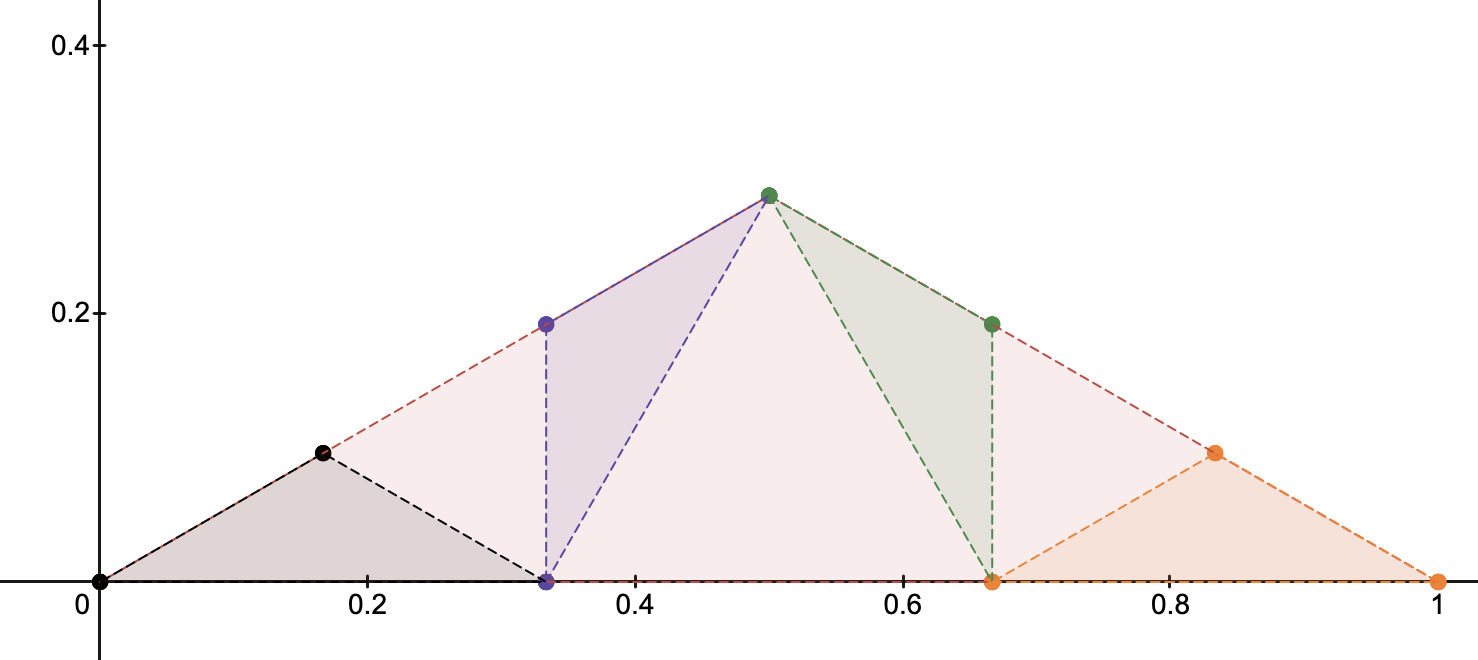
\includegraphics[scale=0.5]{solutions/section-4-1/diag-4-1-2.png}
\end{center}

The contraction ratios are \(c_1 = c_2 = c_3 = c_4 = \frac{1}{3}\) from the definition of a Koch curve.

Therefore, solving
\[
\sum_{i = 1}^{4} \frac{1}{3^s} = 1 \iff 4 = 3^s \iff s = \frac{\log 4}{\log 3},
\]
which means the Hausdorff dimension of the Koch curve is \(\frac{\log 4}{\log 3}\).